% Kozierok, ch. 15
\chapter{IP versions, concepts, and overview}


The Internet Protocol (IP) is a very important protocol in
internetworking. It would be no exaggeration to say that you can't
really comprehend modern networking without a good understanding of IP.
Unfortunately, IP can be somewhat difficult to understand. A large
amount of complexity has become associated with it over the years, and
this has allowed it to meet the many demands placed on it.

Before diving into the details of how IP works, we'll look at the basic
concepts underlying IP. In this chapter, I explain how IP operates in
basic terms and the most important aspects of how it does its job. We'll
look at its main functions, its history, and how it has spawned the
development of several IP-related protocols.



\section{IP overview and key operational characteristics}

IP is the core of the TCP/IP protocol suite and the main protocol at the network layer.
The network layer is primarily concerned with the delivery of data between devices that may be on different networks, which are
interconnected in an arbitrary manner.
In other words, an {\emph{internetwork}}.
IP is the mechanism by which this data is sent on TCP/IP networks (with help from other protocols at the network layer, too, of course).

Let's look at the TCP/IP layer model and consider what IP does from an
architectural standpoint. As the layer~3 protocol, it provides a service
to layer~4 in the TCP/IP stack, represented mainly by the Transmission
Control Protocol (TCP) and User Datagram Protocol (UDP) (see \vref{part:transport-layer}).
IP takes data that has been packaged by either TCP or UDP, manipulates it as necessary, and sends it out (see \cref{fig:ip-main-function}).

This service is sometimes called {\emph{internetwork datagram delivery}}.
There are many details that explain exactly how this service is accomplished, but in a nutshell, IP sends data from point A to point B over an internetwork of connected networks.


\begin{figure}
   \centering
   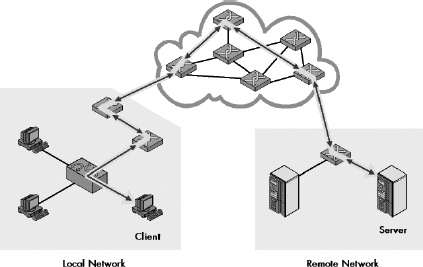
\includegraphics[width=.7\textwidth]{images/ip-main-function.jpg}
   \caption
      [The main function of IP: internetwork datagram delivery]
      {The main function of IP: internetwork datagram delivery --
      IP's overall responsibility is to deliver data between devices on unconnected networks.
      This figure shows how IP delivers datagrams from one device to another over an internetwork;
      in this case, a distant client and server communicate with each other by passing IP datagrams over a series of interconnected networks.}
   \label{fig:ip-main-function}
\end{figure}


\begin{keyconcept}
While the \emph{Internet Protocol} has many functions and characteristics, it can be boiled down to one primary purpose: the delivery of datagrams across an internetwork of connected
networks.
\end{keyconcept}

Of course, there are many ways in which IP could have been implemented in order to accomplish this task.
To understand how the designers of TCP/IP made IP work, let's take a look at the key characteristics used to describe IP and the general manner in which it operates:

\begin{description}
   \item[Universally addressed]
      In order to send data from point A to point B, it is necessary to ensure that devices know how to identify which device is point B.
      IP defines the addressing mechanism for the network and uses these addresses for delivery purposes.

   \item[Underlying protocol-independent]
      IP is designed to allow the transmission of data across any type of underlying network that is designed to work with a TCP/IP stack.
      It includes provisions that allow it to adapt to the requirements of various lower-level protocols such as Ethernet or IEEE 802.11.
      %IP can also run on the special data link protocols, Serial Line Interface Protocol (SLIP) and Point-to-Point Protocol (PPP), that were created for it (see \protect\hyperlink{pt04.html}{Part~II-1}).
      IP can also run on the special data link protocols, SLIP and PPP, that were created for it.
      An important example is IP's ability to fragment large blocks of data into smaller ones in order to match the size limitations of physical networks, and then have the recipient reassemble the pieces again as needed.

   \item[Connectionless delivery]
      IP is a \emph{connectionless} protocol.
      This means that when point A wants to send data to point B, it doesn't first set up a connection to point B and then send the data -- it just makes the datagram and sends it.
      %(See the section in \protect\hyperlink{ch01.html}{Chapter~1} on connection-oriented and connectionless protocols for more information on this.)

   \item[Unreliable delivery]
      IP is said to be an \emph{unreliable} protocol.
      That doesn't mean that one day your IP software will decide to go fishing rather than run your network.
      It does mean that when datagrams are sent from Device A to Device B, Device A just sends each one and then moves on to the next.
      IP doesn't keep track of the ones it sent.
      It does not provide reliability or service-quality capabilities, such as error protection for the data it sends (though it does on the IP header), flow control, or retransmission of lost datagrams.
      For this reason, IP is sometimes called a {\emph{best-effort}} protocol.
      It does what it can to get data to where it needs to go, but makes no guarantees that the data will actually get there.

   \item[Unacknowledged delivery]
      Corresponding with its unreliable nature, IP doesn't use acknowledgements.
      When Device B gets a datagram from Device A, it doesn't send back a ``thank you note'' to tell Device A that the datagram was received.
      It leaves Device A in the dark, so to speak.
\end{description}

These last three characteristics might be enough to make you cringe,
thinking that giving your data to IP would be somewhat like trusting a
new car to your 16-year-old son. If you are going to build an entire
network around this protocol, why design it so that it works without
connections, doesn't guarantee that the data will get there, and has no
means of acknowledging receipt of data?

The reason is simple: Establishing connections, guaranteeing delivery,
error checking, and similar insurance-type functions have
a cost in {\emph{performance}}. It takes time, computer resources, and
network bandwidth to perform these tasks, and they aren't always
necessary for every application. Now, consider that IP carries pretty
much {\emph{all}} user traffic on a TCP/IP network. To build this
complexity into IP would burden all traffic with this overhead, whether
or not it was needed.

The solution taken by the designers of TCP/IP was to exploit the power
of layering. If service-quality features such as connections, error
checking, or guaranteed delivery are required by an application, they
are provided at the transport layer (or possibly, the application
layer). On the other hand, applications that don't need these features
can avoid using them. This is the major distinction between the two
TCP/IP transport layer protocols: TCP and UDP. TCP is full featured but
a bit slower than UDP; UDP is spartan in its capabilities, but faster
than TCP. This system is really the best of both worlds, and it works.



\section{IP functions}

The exact number of IP functions depends on where you draw the line between certain activities.
For explanatory purposes, however, I view IP as having four basic functions (or more accurately, function sets):
\begin{description}
   \item[Addressing]
      Before it can deliver datagrams, IP must know where to deliver them.
      For this reason, IP includes a mechanism for host addressing.
      Furthermore, since IP operates over internetworks, its system is designed to allow for the unique addressing of devices across arbitrarily large networks.
      It also contains a structure to facilitate the routing of datagrams to distant networks, if that is required.
      Since most of the other TCP/IP protocols use IP, an understanding the IP addressing scheme is of vital importance to comprehending much of what goes on in TCP/IP.
      It is explored fully in \cref{chap:kozierok-ch16,chap:kozierok-ch17,chap:kozierok-ch18,chap:kozierok-ch19,chap:kozierok-ch20}.

   \item[Data encapsulation and formatting/packaging]
      As the TCP/IP network layer protocol, IP accepts data from the transport layer protocols UDP and TCP.
      It then encapsulates this data into an IP datagram using a special format prior to transmission.

   \item[Fragmentation and reassembly]
      IP datagrams are passed down to the data link layer for transmission on the local network.
      However, the maximum frame size of each physical and data link network using IP may be different.
      For this reason, IP includes the ability to {\emph{fragment}} IP datagrams into pieces, so that they can each be carried on the local network.
      The receiving device uses the {\emph{reassembly}} function to re-create the whole IP datagram.
      Some people view fragmentation and reassembly as distinct functions, though clearly they are complementary, and I view them as being part of the same job.
      Fragmentation and reassembly are discussed in \vref{chap:kozierok-ch22}.

   \item[Routing and indirect delivery]
      When an IP datagram must be sent to a destination on the same local network, you can do this easily with the network's underlying local area network (LAN), wireless LAN (WLAN), or wide area network (WAN) protocol, using what is sometimes called {\emph{direct delivery}}.
      However, in many (if not most cases) the final destination is on a distant network that isn't directly attached to the source.
      In this situation, the datagram must be delivered indirectly.
      This is accomplished by routing the datagram through intermediate devices ({\emph{routers}}).
      IP accomplishes this in concert with support from the other protocols including the Internet Control Message Protocol (ICMP) and the TCP/IP gateway/routing protocols such as the Routing Information Protocol (RIP) and the Border Gateway Protocol (BGP).
\end{description}


\section{IP history, standards, versions, and closely related protocols}

Since IP is really the architectural foundation for the entire TCP/IP
protocol suite, you might have expected that it was created first, and
that the other protocols were built upon it. That's usually how you
build a structure, after all! The history of IP, however, is a bit more
complex. The functions it {\emph{performs}} were defined at the birth of
the protocol, but IP itself didn't exist for the first few years that
the protocol suite was being
defined.

I explore the early days of TCP/IP in \protect\hyperlink{ch08.html}{Chapter~8}, which provides an overview of the suite as a whole.
What is notable about the development of IP is that its functions were originally part of TCP.
As a formal protocol, IP was born when an early version of TCP developed in the 1970s for predecessors of the modern Internet was split into TCP at layer~4 and IP at layer~3.
The key milestone in the development of IP was the publication of RFC 791, ``Internet Protocol,'' in September 1981.
This standard, a revision of the similar RFC 760 of the previous year, defined the core functionality and characteristics of the version of IP that has been in widespread use for the last two decades.



\subsection{IP versions and version numbers}

The IP defined in RFC 791 was the first widely used version of IP.
Interestingly, however, it is not version 1 of IP but version 4! This would of course imply that there were earlier versions of the protocol at one point.
Interestingly, however, there really weren't.
IP was created when its functions were split out from an early version of TCP that combined both TCP and IP functions.
TCP evolved through three earlier versions and was split into TCP and IP for version 4.
That version number was applied to both TCP and IP for consistency.

\begin{keyconcept}
Version 4 of the \emph{Internet Protocol} is actually the first version that was widely deployed and is currently the one in widespread use.
\end{keyconcept}

So, when you use IP today, you are using IP version 4, which is
frequently abbreviated IPv4. Unless otherwise qualified, it's safe to
assume that {\emph{IP}} means IP version 4 -- at least for the next few years.
(This version number is carried in the appropriate field of all IP datagrams, as described in the topic discussing the IP datagram format in \vref{chap:kozierok-ch21}.)

Given that it was originally designed for an internetwork a tiny
fraction of the size of our current Internet, IPv4 has proven itself remarkably capable.
Various additions and changes have been made over
time to how IP is used, especially with respect to addressing, but the
core protocol is basically what it was in the early 1980s. There's good
reason for this. Changing something as fundamental as IP requires a
great deal of development effort and also introduces complexities during
transition.

IPv4 has served us well, but people understood that, for various
reasons, a new version of IP would eventually be required. Due to the
difficulties associated with making such an important change,
development of this new version of IP has actually been under way since
the mid-1990s. This new version of IP is formally called {\emph{Internet
Protocol version 6 (IPv6)}} and also sometimes referred to as {\emph{IP
Next Generation}} or {\emph{IPng}}.
I discuss the reasons why IPv6 was developed and how it differs from IPv4 in considerable detail in \vref{chap:ipv6}.

A natural question at this point is, ``What happened to version 5 of IP?''
The answer is that it doesn't exist. While this may seem confusing,
version 5 was in fact intentionally skipped in order to {\emph{avoid}}
confusion, or at least to rectify it. The problem with version 5 relates
to an experimental TCP/IP protocol called the {\emph{Internet Stream
Protocol, version 2}}, originally defined in RFC 1190. This protocol was
originally seen by some as being a peer of IP at the Internet layer in
the TCP/IP architecture, and in its standard version, these packets were
assigned IP version 5 to differentiate them from normal IP packets
(version 4). This protocol apparently never went anywhere, but to be
absolutely sure that there would be no confusion, version 5 was skipped
over in favor of version 6.




\subsection{IP-related protocols}


In addition to the old and new versions of IP, there are several protocols that are {\emph{IP-related}}.
These are protocols that add to or expand on the capabilities of IP functions for special circumstances, but they are not part of IP proper.
These are as follows:
\begin{description}
   \item[Network address translation]
      This protocol\footnote{NAT is not a protocol. Kozierok is wrong here.} provides IP address translation capabilities that allow private networks to be interfaced to public networks in a flexible manner.
      It allows public IP addresses to be shared and improves security by making it more difficult for hosts on the public network to gain unauthorized access to hosts.
      It is commonly called {\emph{NAT}}.
      This protocol is discussed in \vref{chap:nat}.

   \item[IPsec]
      IPsec defines a set of subprotocols that provide a mechanism for the secure transfer of data using IP.
      It is rapidly growing in popularity as a security protocol that enables virtual private networks.
      This protocol\footnote{IPsec can better be described as a set of protocols or a framework.} is discussed in \protect\hyperlink{ch29.html}{Chapter~29}.

   \item[Mobile IP]
      This is a protocol that addresses some of the difficulties associated with using IP on computers that frequently move from one network to another.
      It provides a mechanism that allows data to be automatically routed to a mobile host (such as a notebook computer), without requiring a constant reconfiguration of the device's IP address.
      This protocol is discussed in \protect\hyperlink{ch30.html}{Chapter~30}.
\end{description}
